\documentclass[letterpaper,twocolumn,9pt]{extarticle}
\usepackage[T1]{fontenc}
\usepackage[utf8]{inputenc}
\usepackage[letterpaper,top=0.67in,bottom=0.67in,left=0.69in,right=0.69in,columnsep=0.19in]{geometry}
\usepackage{times}
\usepackage{amsmath,amssymb,amsfonts}
\usepackage{graphicx}
\usepackage{booktabs}
\usepackage{multirow}
\usepackage{url}
\usepackage{xcolor}
\usepackage{cite}
\usepackage[compact]{titlesec}
\usepackage{caption}
\usepackage{microtype}
\usepackage{array}
\usepackage{enumitem}
\captionsetup{labelsep=period,font=small,justification=centering,skip=4pt}
\captionsetup[figure]{name=Fig.}
\captionsetup[table]{name=TABLE}
\graphicspath{{figures/}}

\setlength{\parindent}{0.167in}
\setlength{\parskip}{0pt}
\setlength{\textfloatsep}{8pt plus 2pt minus 2pt}
\setlength{\floatsep}{7pt plus 2pt minus 2pt}
\setlength{\intextsep}{7pt plus 2pt minus 2pt}
\setlength{\abovecaptionskip}{4pt}
\setlength{\belowcaptionskip}{2pt}
\setlist[itemize]{leftmargin=1.3em,itemsep=2pt,topsep=3pt}
\pagestyle{empty}
\renewcommand{\thesection}{\Roman{section}}
\renewcommand{\thesubsection}{\Alph{subsection}}
\renewcommand{\thesubsubsection}{\arabic{subsubsection})}
\titleformat{\section}[block]{\centering\fontsize{11}{13}\selectfont\scshape}{\thesection.}{0.5em}{}
\titlespacing*{\section}{0pt}{8pt}{5pt}
\titleformat{\subsection}[block]{\itshape\fontsize{9.5}{11}\selectfont}{\thesubsection.}{0.5em}{}
\titlespacing*{\subsection}{0pt}{6pt}{3pt}
\titleformat{\subsubsection}[runin]{\itshape}{\thesubsubsection}{0.4em}{}[.]
\titlespacing*{\subsubsection}{0pt}{4pt}{0.5em}

\newcommand{\Cps}{C_{ps}}
\newcommand{\Lp}{L_p}
\newcommand{\Ls}{L_s}
\newcommand{\Mut}{M}
\newcommand{\Rac}{R_{ac}}
\newcommand{\Rdc}{R_{dc}}
\newcommand{\etal}{\emph{et al.}}

\begin{document}

\twocolumn[{%
\centering
{\fontsize{16}{19}\selectfont\bfseries Solver-Supervised Graph Neural Surrogates for Parasitic Extraction and Layout Screening in PCB Planar Magnetics\par}
\vspace{9pt}
{\fontsize{10}{12}\selectfont Duong Viet Hoang$^{1,*}$, \quad Lun-Min Shih$^{1}$\par}
\vspace{3pt}
{\fontsize{9}{11}\selectfont $^{1}$Department of Computer Science, Da-Yeh University, Taiwan\par}
{\fontsize{9}{11}\selectfont Hoangduong4316@icloud.com, \quad Lmshih@mail.dyu.edu.tw \quad ($^{*}$Corresponding author)\par}
\vspace{9pt}
}]

\noindent\textbf{Abstract}---PCB-embedded planar magnetics compress a converter but make winding parasitics unusually sensitive to foil placement, layer order, and lateral registration. Closed-form partial-element approximations are fast enough for a design loop, yet they can miss the same three-dimensional effects that the designer is trying to control. Full field extraction has the opposite problem. This paper develops a geometry-aware graph surrogate for the inter-winding capacitance $\Cps$, the two free-space winding self-inductances $\Lp$ and $\Ls$, and the winding mutual inductance $\Mut$. The training labels are regenerated with a three-dimensional electrostatic finite-element solve for $\Cps$ and FastHenry for the inductive quantities. On a held-out field-solver corpus, median errors are 3.22, 2.83, 3.81, and 2.56\%, respectively, whereas the replaced analytical labels differ from those references by 51.5--266.6\%. An independent Neumann-integral implementation places the learned inductive estimates within the spread between two solver formulations. A pairwise head addresses a separate design question: ordering variants of an unseen layout. It raises family-disjoint Spearman correlation from 0.27 for pointwise regression to 0.93 and, on lateral registration where the analytical capacitance is constant, reduces selection regret from 1176.1 to 3.5\%.

The expanded study also separates properties that were previously easy to conflate. A corrected coordinate-update network is strictly $E(3)$-equivariant on the encoded graph: maximum transformed-output and coordinate residuals are $4.38\times10^{-7}$ and $1.42\times10^{-7}$. Its accuracy effect against a parameter-matched invariant distance-message network is nevertheless unresolved ($-0.007$\%, 95\% confidence interval $[-8.98,8.98]$\%); the interval also fails a predeclared $\pm2$\% practical-equivalence criterion. Finally, measured latency is reported at three boundaries. The median is 0.64\,ms/design for pre-collated batch throughput, 2.37\,ms for a single forward pass, and 5.90\,ms from raw layout through graph construction and inference, versus 4.17\,s for the paired field-solvers. The corresponding paired end-to-end speedup is $735\times$ (95\% confidence interval $682$--$796\times$). These results establish a solver-grade screening tool, not a hardware-calibrated extractor; fabricated-board validation remains necessary.

\vspace{4pt}
\noindent\textbf{Index Terms}---Graph neural network, parasitic extraction, planar magnetics, partial-element equivalent circuit, finite element method, layout optimization, equivariance.

\section{Introduction}
Planar transformers and inductors replace wound wire with copper foils patterned across a printed-circuit stack. Their low profile and repeatable geometry suit high-density GaN and SiC converters, but the same construction couples the windings over broad overlapping areas. Inter-winding capacitance drives common-mode current, while self and mutual inductance shape leakage, ringing, and energy transfer. At high switching slew rates, moving one foil or changing one layer can alter the electromagnetic behavior enough to change the preferred layout~\cite{ouyang,hurley,ott}.

The practical tension is familiar. Closed-form strip and parallel-plate models return an answer almost immediately. They are useful for hand calculation and early sizing, but their compactness comes from assumptions about current distribution, fringing, and overlap. Three-dimensional solvers resolve more of the geometry, at a cost that makes an exhaustive inner-loop search unattractive. A learned surrogate can occupy the gap only if its labels reflect the field solution. Matching a cheap approximation more accurately does not repair the approximation.

This work begins with that distinction. An analytical partial-element model was first used to generate a large synthetic corpus. It produced a clean machine-learning benchmark, but comparison with field solvers exposed substantial label error. The revised pipeline regenerates the capacitance with an electrostatic volume FEM and the inductance matrix with FastHenry. A message-passing graph neural network (GNN) is then trained on those solver outputs. The graph representation preserves variable conductor count and exposes pair geometry to a shared message function. It also supports a sparse $k$-nearest-neighbor form when the all-pairs graph becomes unnecessarily expensive.

The expanded study answers five questions that are distinct in an actual design flow:
\begin{itemize}
\item How far are the convenient analytical labels from three-dimensional references, and does relabeling close that gap?
\item Does graph structure earn its cost relative to pooled multilayer perceptrons and gradient-boosted trees?
\item Can the model rank close variants within an unseen design family, not merely predict well over a heterogeneous test set?
\item Is strict rigid-motion symmetry present in the implementation, and does the coordinate update improve accuracy or sample efficiency?
\item What speedup remains when graph construction and batch size are stated explicitly?
\end{itemize}

The answer is not uniformly favorable to the more elaborate model. Message passing is valuable for the relational inductive targets and for transfer across graph size. Pairwise training is valuable for ordering. By contrast, the strict equivariant coordinate update has no resolved advantage in the parameter-matched experiment, and the uncertainty is too wide to call the two models equivalent. Likewise, the dense graph does not beat the analytical code at the small benchmark size; its use is justified by solver-level accuracy rather than raw speed against a lower-fidelity approximation.

Figure~\ref{fig:pipeline} summarizes the scope. The predicted vector is $[\Cps,\Lp,\Ls,\Mut]$. Here $\Mut$ denotes winding mutual inductance in free space. It is not the ferrite-core magnetizing inductance, which depends on the magnetic circuit and is much larger in the operating component. Nor is the output a complete broadband RLGC matrix. These boundaries matter when interpreting both accuracy and deployment.

\begin{figure*}[t]
\centering
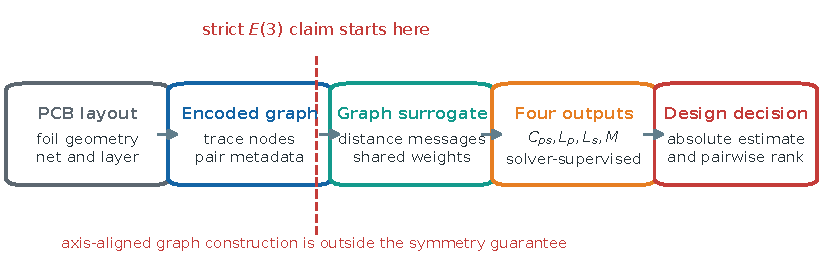
\includegraphics[width=0.98\textwidth]{fig1_pipeline_scope.pdf}
\caption{From layout to design decision. The strict $E(3)$ statement applies after the layout has been encoded as a graph. The current graph builder uses axis-aligned overlap metadata and is not part of that guarantee. The regression and pairwise heads answer different questions: absolute parasitic estimation and ordering within a candidate family.}
\label{fig:pipeline}
\end{figure*}

\section{Related Work}
\subsection{Parasitic Extraction for Planar Windings}
The partial-element equivalent-circuit (PEEC) method converts electromagnetic interactions into circuit quantities~\cite{ruehli}. Closed-form inductance expressions such as Grover's formulas remain useful for rapid estimates~\cite{grover}, while FastHenry assembles and accelerates a three-dimensional partial-inductance solve~\cite{fasthenry}. For capacitance, FastCap introduced multipole-accelerated boundary-element extraction~\cite{fastcap}; finite-element formulations offer an alternative when thin gaps or panel conditioning make a surface discretization difficult. Winding-resistance models trace back to Dowell and related treatments of skin and proximity effect~\cite{dowell,kazimierczuk}.

The present work does not propose a new field solver. Its contribution is a learned approximation to solver outputs over a constrained family of multilayer foil geometries. That distinction separates numerical fidelity of the references from generalization of the surrogate.

\subsection{Graph Learning for Physical and EDA Problems}
Message-passing networks represent a system as entities connected by learned interactions~\cite{gilmer,battaglia}. They have been used to learn physical dynamics~\cite{sanchez,pfaff}, IC placement and sizing~\cite{mirhoseini,gcnrl}, net-length estimation~\cite{net2}, and layout-dependent parasitics~\cite{paragraph,circuitgnn}. Graphs are attractive here because conductor count varies and the targets accumulate pair interactions.

Rigid-motion-aware networks place a stronger constraint on those interactions. In an EGNN, scalar messages depend on invariant quantities such as squared distance, and coordinate updates are scalar-weighted relative vectors~\cite{egnn}. This construction is exact only if every learned message input respects the assumed group action. Raw Cartesian components passed to an unconstrained scalar MLP break that premise. We therefore treat strict symmetry as a testable implementation property rather than infer it from the architecture's name.

\subsection{Prediction Versus Ranking}
An optimizer often needs the best candidate rather than a calibrated value for every candidate. Pointwise regression and learning to rank are not interchangeable objectives. RankNet and later ranking methods train on relative order or pairwise margins~\cite{ranknet,lambdamart}. The distinction is important when the between-family range is much larger than the variation among candidates in one family: high global $R^2$ can coexist with poor within-family ordering.

\section{Problem Definition and Physical Scope}
\subsection{Layout and Targets}
A layout contains rectangular copper traces indexed by $i=1,\ldots,N$. Each trace has a net assignment, layer, center coordinate $x_i\in\mathbb{R}^3$, width $w_i$, length $\ell_i$, thickness $t_i$, conductivity $\sigma_i$, and surrounding dielectric description. Primary and secondary turns are series-connected. We predict four extensive scalars,
\begin{equation}
y=\left[\Cps,\Lp,\Ls,\Mut\right],
\end{equation}
where $\Cps$ is total primary-to-secondary capacitance, $\Lp$ and $\Ls$ are the free-space series self-inductances of the two windings, and $\Mut$ is their winding mutual inductance.

FastHenry returns a partial-inductance matrix rather than the series winding quantity directly. If $\mathcal{P}$ indexes primary traces, the consistent composition is
\begin{equation}
\Lp=\sum_{i\in\mathcal{P}}L_{ii}+2\sum_{\substack{i,j\in\mathcal{P}\\i<j}}L_{ij},
\label{eq:seriesL}
\end{equation}
with analogous expressions for $\Ls$ and the cross-winding sum $\Mut$. The surrogate is trained on these compositions, not on individual matrix entries.

The magnetic core is deliberately excluded. The operating transformer inductance includes a magnetizing term set by permeability, gap, and core geometry. A separate core calculation found that term to be roughly 37--73 times the free-space winding mutual over representative layouts. Thus $\Mut$ is a geometric winding quantity, not a substitute for magnetizing inductance.

\subsection{Solver-Grade Rather Than Hardware-Grade}
``Solver-grade'' in this paper has a narrow meaning: held-out predictions are compared with the designated three-dimensional numerical references. It does not mean that a fabricated PCB was measured, that copper roughness and manufacturing tolerance were calibrated, or that the electrostatic model captures every layered-dielectric detail. A cross-solver inductance check reduces the risk of learning one program's numerical idiosyncrasies, but two numerical formulations may still share modeling assumptions.

\subsection{Symmetry Boundary}
Let $Q\in O(3)$ and $t\in\mathbb{R}^3$. A rigid transform acts on encoded node coordinates as
\begin{equation}
x_i\mapsto Qx_i+t.
\end{equation}
The four targets are invariant scalars. Updated coordinates inside an equivariant network should transform by the same action. Stored scalar metadata, including edge type and precomputed overlap, is held fixed in this test.

This is an encoded-graph statement. The layout-to-graph routine computes axis-aligned overlap before the transform. Rotating a raw layout and recomputing that overlap need not yield the same graph. Calling the entire raw-layout pipeline strictly equivariant would therefore be incorrect.

\section{Reference Solvers and Data}
\subsection{Analytical Teacher and Its Audit}
The initial teacher accumulates pairwise strip-inductance and capacitance approximations. Its speed made it useful for early architecture studies on 2000 layouts, and the GNN reproduced that teacher with $R^2>0.999$. That result measures teacher fidelity. It is not evidence of agreement with a field solution.

The discrepancy became visible when the same layouts were evaluated with independent references. Median analytical error was 51.5\% for $\Lp$, 53.6\% for $\Ls$, and 58.6\% for $\Mut$ against FastHenry. For $\Cps$, an overlap formula based on dimensions but not lateral offset differed from the electrostatic FEM by 266.6\%. The capacitance failure is especially instructive: two traces of equal dimensions can have identical analytical capacitance whether stacked or laterally disjoint, even though their true coupling changes sharply.

\subsection{Inductance Reference}
FastHenry discretizes each conductor cross-section and solves for the three-dimensional partial-inductance matrix~\cite{fasthenry}. The entries are composed according to (\ref{eq:seriesL}). Every valid layout supplies $\Lp$, $\Ls$, and $\Mut$. Positive mutual inductance and a completed matrix are required for inclusion.

An independent reference evaluates the Neumann double integral using a $5\times2$ filament subdivision. It shares neither the FastHenry executable nor its linear-system implementation. Across 70 held-out layouts, the GNN versus Neumann median errors are 6.61, 4.96, and 2.03\% for $\Lp$, $\Ls$, and $\Mut$; FastHenry versus Neumann gives 4.95, 4.78, and 2.07\%. The learned $\Mut$ therefore lies within the inter-solver discrepancy, while $\Lp$ retains a modest additional model error.

\subsection{Capacitance Reference}
The electrostatic reference solves
\begin{equation}
\nabla\!\cdot\!\left(\epsilon\nabla\phi\right)=0
\end{equation}
on a tetrahedral volume mesh with primary and secondary conductors held at 1 and 0\,V. The capacitance follows from stored field energy $W$,
\begin{equation}
\Cps=\frac{2W}{V^2}.
\end{equation}
The volume formulation was chosen after surface-panel experiments proved unstable at the approximately 0.1\,mm inter-layer gaps. A stacked pair and a 60\,mm-offset pair yielded 92.9 and 0.38\,pF in the volume solve, whereas the position-blind analytical expression assigned both 44.3\,pF.

\subsection{Corpora and Splits}
The field-accuracy experiment contains 332 valid designs and uses a 265/67 train/test split. The strict-equivariance ablation independently regenerates the same number of valid designs from 346 attempts and fixes a 266/66 split across every architecture and initialization. These two experiments are reported separately; their test indices are not silently pooled. Training statistics are fitted only on the active training subset.

The layouts are synthetic eight-layer planar-LLC winding geometries. They vary trace count, dimensions, layer assignment, interleaving, and lateral registration. The field corpus reaches 70 trace nodes. No via, return-plane, connector, or measured process-variation model is included.

\begin{table}[t]
\caption{Experimental corpora and the question each answers.}
\label{tab:corpora}
\centering
\footnotesize
\setlength{\tabcolsep}{3.5pt}
\begin{tabular}{p{0.21\columnwidth}rrrrp{0.31\columnwidth}}
\toprule
Experiment & valid & train & test & seeds & purpose\\
\midrule
Field accuracy & 332 & 265 & 67 & 1 & four-target solver agreement\\
Strict $E(3)$ & 332 & 266 & 66 & 5 & symmetry, accuracy effect, sample efficiency\\
Ranking & 880 & 77 fam. & 33 fam. & 1 & family-disjoint ordering\\
Frequency & 136 & 109 & 27 & 1 & $\Rac/\Rdc(f)$ extension\\
\bottomrule
\end{tabular}
\end{table}

\section{Graph Surrogates}
\subsection{Encoded Graph}
Each trace becomes a node. Invariant node scalars are width, length, thickness, log conductivity, relative permittivity, and normalized layer. Directed edges connect either all trace pairs or the $k$ nearest neighbors. For the audited invariant/strict comparison, learned messages receive overlap and coupling-type flags plus a distance recomputed from coordinates. Raw $\Delta x$, $\Delta y$, and $\Delta z$ components are not sent to an unconstrained scalar MLP.

The dense graph has $O(N^2)$ edges and mirrors the all-pairs reference. The sparse graph has $O(Nk)$ edges. Since magnetic and electric coupling decay with separation, local neighborhoods retain much of the predictive signal. The asymptotic saving matters only after graph construction and inference dominate other fixed costs.

\subsection{Invariant Distance-Message Network}
Let $h_i^{(\ell)}$ denote the hidden scalar state at layer $\ell$, $a_{ij}$ invariant edge metadata, and $r_{ij}^{(\ell)}=\|x_i^{(\ell)}-x_j^{(\ell)}\|^2$. A message and node update are
\begin{align}
m_{ij}^{(\ell)}&=\phi_m\!\left(h_i^{(\ell)},h_j^{(\ell)},r_{ij}^{(\ell)},a_{ij}\right),\\
h_i^{(\ell+1)}&=\operatorname{LN}\!\left[h_i^{(\ell)}+\phi_h\!\left(h_i^{(\ell)},\operatorname{mean}_{j}m_{ji}^{(\ell)}\right)\right].
\end{align}
The invariant baseline keeps $x_i^{(\ell+1)}=x_i^{(\ell)}$. Four layers are followed by mean, max, and signed-log-sum pooling. Their concatenation enters a four-output head. The sum channel is useful because the targets are extensive.

\subsection{Strict Coordinate-Update Network}
The strict model uses the identical scalar path and adds
\begin{equation}
x_i^{(\ell+1)}=x_i^{(\ell)}+\operatorname{mean}_{j}\left[
\frac{x_i^{(\ell)}-x_j^{(\ell)}}{\sqrt{r_{ij}^{(\ell)}}+1}
c\!\left(m_{ij}^{(\ell)}\right)\right],
\label{eq:coord}
\end{equation}
where $c(\cdot)$ is an invariant learned scalar bounded by a scaled hyperbolic tangent. Because the multiplier is invariant and the displacement is a relative vector, (\ref{eq:coord}) is equivariant to rotations, reflections, and translations. Scalar pooling makes the graph output invariant.

The strict width-96 network has 310,763 trainable parameters. The primary invariant comparison uses width 102 and 307,945 parameters, a 0.91\% difference. A width-96 invariant network with 273,127 parameters supplies a sensitivity comparison. Widening only the baseline is not a perfect control for optimization, so both comparisons are retained.

\subsection{Pairwise Ranking Head}
For candidates $a$ and $b$ from one design family, the ranking head produces scores $s_a,s_b$ and minimizes a margin loss,
\begin{equation}
\mathcal{L}_{\mathrm{rank}}=\max\left(0,\gamma-z_{ab}(s_a-s_b)\right),
\end{equation}
where $z_{ab}\in\{-1,1\}$ encodes the solver ordering. Families, rather than individual layouts, are assigned to train or test. This prevents variants of the same base geometry from leaking across the split.

\section{Experimental Protocol}
\subsection{Training and Metrics}
All networks use AdamW, learning rate $2\times10^{-3}$ with cosine decay, weight decay $10^{-5}$, batch size 32, gradient-norm clipping at 5, and SmoothL1 loss on standardized signed-$\log(1+|y|)$ targets. Scalar feature and target moments are estimated from training data only. Coordinates are divided by one isotropic training-derived scale; separate axis scales would destroy exact rotational symmetry.

The primary EGNN metric is a per-design macro error,
\begin{equation}
e_i=\frac{1}{4}\sum_{q=1}^{4}\left|\log(1+\hat y_{iq})-\log(1+y_{iq})\right|.
\end{equation}
It avoids giving the largest-magnitude target automatic control of the comparison. Per-target $R^2$ and median relative error remain secondary descriptive metrics.

The strict ablation fixes one test set and five initialization/training-order seeds. Nested training sizes are 25, 50, 100, 200, and the full 266 designs. Uncertainty uses 10,000 paired hierarchical bootstrap resamples: seeds are resampled first and held-out designs second. The relative effect is strict minus invariant; negative values favor strict EGNN. Practical equivalence was defined before inspecting results as a 90\% interval entirely inside $[-2,2]$\%. A directional practical effect requires the 95\% interval to clear the corresponding $\pm2$\% boundary.

\subsection{Symmetry Test}
Each full-data strict model is evaluated under proper rotations, reflections, and translations. The test compares invariant outputs and equivariant coordinates against their transformed expectations. Relative tolerance is $2\times10^{-5}$. The five models contribute 200 transformed cases. Failure of any full-data seed blocks a strict-symmetry claim.

\subsection{Latency Boundaries}
Latency can change by nearly an order of magnitude without changing the network, simply by moving the timer. We therefore report:
\begin{enumerate}[leftmargin=1.4em,itemsep=1pt,topsep=3pt]
\item \emph{pre-collated batch throughput}: one prepared test batch divided by batch size;
\item \emph{single forward}: a prepared graph evaluated alone;
\item \emph{raw-layout end to end}: graph construction, normalization, collation, forward pass, and inverse target transform;
\item \emph{paired solver}: FastHenry plus the electrostatic FEM for the same design.
\end{enumerate}
The primary speedup pairs each design's solver time with its end-to-end GNN time and bootstraps the median ratio. Throughput is useful for screening a large candidate bank but is not substituted for batch-one latency.

\section{Results}
\subsection{Field-Solver Accuracy}
Relabeling changes the result more than changing the architecture. Figure~\ref{fig:field} compares the analytical discrepancy with the held-out solver-supervised GNN error. The improvement spans all four targets. Capacitance falls from 266.6 to 3.22\% median error; the three inductive quantities fall from 51.5--58.6 to 2.56--3.81\%. Table~\ref{tab:field} gives the corresponding $R^2$ values.

\begin{figure}[t]
\centering
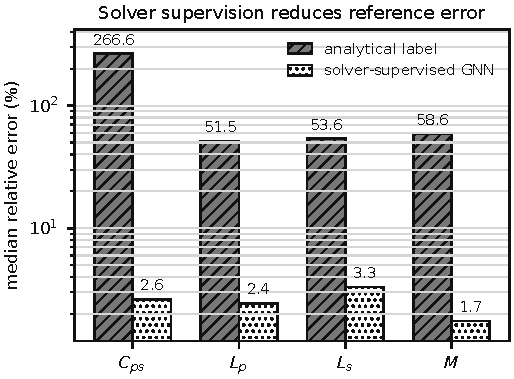
\includegraphics[width=0.98\columnwidth]{fig2_field_accuracy.pdf}
\caption{Median relative error against the designated three-dimensional reference. Analytical values are teacher errors; GNN values are held-out prediction errors after relabeling. The logarithmic axis keeps the four improvements visible without hiding their different scales.}
\label{fig:field}
\end{figure}

\begin{table}[t]
\caption{Held-out field-solver accuracy (332 valid layouts; 265/67 split).}
\label{tab:field}
\centering
\small
\begin{tabular}{lccc}
\toprule
Target & reference & median error & $R^2$\\
\midrule
$\Cps$ & electrostatic FEM & 3.22\% & 0.9527\\
$\Lp$ & FastHenry & 2.83\% & 0.9954\\
$\Ls$ & FastHenry & 3.81\% & 0.9942\\
$\Mut$ & FastHenry & 2.56\% & 0.9943\\
\bottomrule
\end{tabular}
\end{table}

The capacitance $R^2$ is lower than the inductive values even though its typical relative error is similar. This is not contradictory. $R^2$ is dominated by squared residuals and the high-capacitance tail, whereas the median relative error weights a typical design. Reporting both prevents a favorable scalar from obscuring a different failure mode.

\subsection{Why Use a Graph?}
Table~\ref{tab:trees} compares the GNN with four tree ensembles built from the same pooled 27-dimensional summary on an identical 332/67 solver-labeled split. LightGBM slightly improves the typical $\Cps$ relative error (2.9 versus 3.2\%), while the GNN has higher $R^2$ (0.953 versus 0.942). A graph is not necessary to obtain a competitive scalar capacitance predictor.

The picture changes for relational quantities. Tree $R^2$ remains between 0.878 and 0.920 on the inductances, while the GNN reaches 0.994--0.995. On a graph-size extrapolation split, tree $R^2(\Mut)$ falls to 0.112--0.324; the GNN retains 0.943. The shared message function applies without redesign when trace count changes. A pooled MLP likewise reproduced scalar capacitance but degraded toward $R^2\approx0.88$ on $\Lp$ and $\Ls$. These controls identify pairwise geometry, rather than parameter count alone, as the useful inductive bias.

\begin{table*}[t]
\caption{Tree baselines and GNN on the identical field-solver split. Parentheses contain median relative error in percent. Rank $\rho$ is reported only where a family-disjoint ranking experiment exists; size transfer is $R^2(\Mut)$.}
\label{tab:trees}
\centering
\small
\setlength{\tabcolsep}{6pt}
\begin{tabular}{lrrrrrr}
\toprule
Model & $\Cps$ & $\Lp$ & $\Ls$ & $\Mut$ & rank $\rho$ & size transfer\\
\midrule
Random Forest & .462 (12.9) & .887 (24.8) & .914 (15.9) & .880 (9.3) & --- & .112\\
XGBoost & .927 (3.8) & .878 (16.3) & .908 (16.5) & .914 (7.8) & --- & .231\\
LightGBM & .942 (\textbf{2.9}) & .893 (23.9) & .890 (20.2) & .918 (7.1) & .088 & .247\\
CatBoost & .892 (4.7) & .896 (24.5) & .893 (20.4) & .920 (8.1) & --- & .324\\
\textbf{GNN} & \textbf{.953} (3.2) & \textbf{.995} (\textbf{2.8}) & \textbf{.994} (\textbf{3.8}) & \textbf{.994} (\textbf{2.6}) & \textbf{.929} & \textbf{.943}\\
\bottomrule
\end{tabular}
\end{table*}

\subsection{Strict $E(3)$: Verified Symmetry, Unresolved Accuracy Effect}
All five strict models pass the transformation gate. Across 200 cases, the maximum relative residual is $4.38\times10^{-7}$ for graph outputs and $1.42\times10^{-7}$ for updated coordinates, more than an order of magnitude below the $2\times10^{-5}$ tolerance. This establishes strict $E(3)$ behavior on the encoded graph, including reflections.

Symmetry verification does not imply a predictive gain. On the full training set, the primary error is 0.028886 for strict EGNN and 0.028888 for the parameter-matched invariant model. The relative change is $-0.007$\%, with 95\% CI $[-8.98,8.98]$\%. The 90\% interval $[-7.50,7.61]$\% is not contained in the predeclared $\pm2$\% equivalence region. Neither improvement nor practical equivalence is established.

The same-width sensitivity arm favors the invariant network: strict EGNN error is 12.77\% higher, 95\% CI $[2.25,24.46]$\%. Because this baseline has fewer parameters, the result should not replace the parameter-matched primary analysis. It does show that the coordinate update does not produce a robust advantage merely by adding capacity. Figure~\ref{fig:egnn} displays both comparisons.

Sample efficiency is similarly unresolved. The normalized area under error versus $\log_2(n_{\mathrm{train}})$ is 1.91\% higher for strict EGNN, 95\% CI $[-1.23,4.42]$\%. Individual training sizes change direction, which is why a learning curve and paired seeds are more informative than a selected single run.

\begin{figure*}[t]
\centering
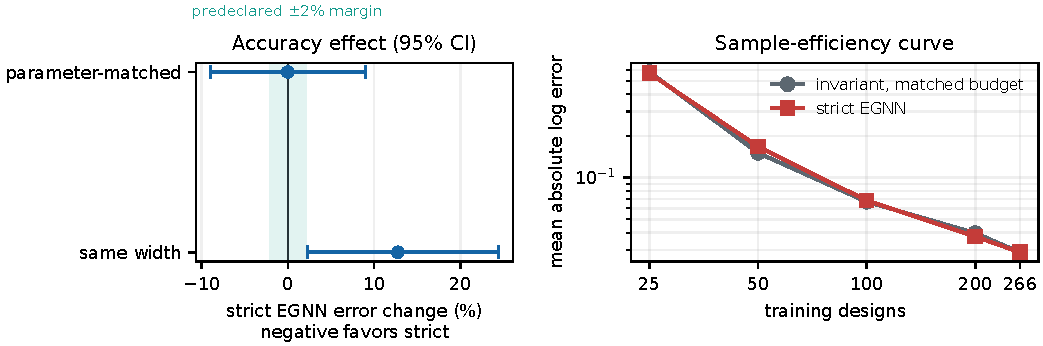
\includegraphics[width=0.96\textwidth]{fig3_strict_e3_ablation.pdf}
\caption{Strict-coordinate-update ablation. Left: relative primary-error effects with paired hierarchical-bootstrap 95\% intervals; the shaded band is the predeclared practical-equivalence margin. Right: five-seed mean learning curves on one fixed split. Exact encoded-graph symmetry is verified, but its accuracy and sample-efficiency effects are unresolved in the parameter-matched comparison.}
\label{fig:egnn}
\end{figure*}

\begin{table}[t]
\caption{Controlled strict-$E(3)$ ablation (five seeds, fixed 266/66 split). Positive error change favors the invariant model.}
\label{tab:egnn}
\centering
\footnotesize
\begin{tabular}{p{0.42\columnwidth}rr}
\toprule
Comparison & effect & 95\% CI\\
\midrule
Full, parameter matched & $-0.007$\% & $[-8.98,8.98]$\\
Full, same width & $+12.77$\% & $[2.25,24.46]$\\
Sample-efficiency AULC & $+1.91$\% & $[-1.23,4.42]$\\
\midrule
Output residual, max & \multicolumn{2}{r}{$4.38\times10^{-7}$}\\
Coordinate residual, max & \multicolumn{2}{r}{$1.42\times10^{-7}$}\\
\bottomrule
\end{tabular}
\end{table}

\subsection{Ranking and Design Regret}
The pointwise field-accuracy model orders variants of unseen families at only $\rho=0.27$. A dedicated pairwise head raises median family-disjoint $\rho$ to 0.929 across 33 test families. The gap is not a paradox: global error is dominated by differences among base designs, while an optimizer compares much smaller changes within one family.

Two layout levers illustrate where learning matters. For layer-order interleaving, the analytical model already sees vertical spacing and reaches $\rho=0.78$; the GNN reaches 0.81, and both select low-regret candidates (5.4 and 5.8\%). For lateral registration, the analytical overlap expression is constant in every test family and cannot rank at all. The GNN reaches $\rho=0.95$. When asked to select the minimum-$\Cps$ candidate, analytical screening incurs 1176.1\% regret relative to the FEM optimum, similar to random selection at 1126.2\%; GNN screening reduces it to 3.5\% (Fig.~\ref{fig:rank}). This is the layout lever for which three-dimensional supervision changes the decision.

\begin{figure*}[t]
\centering
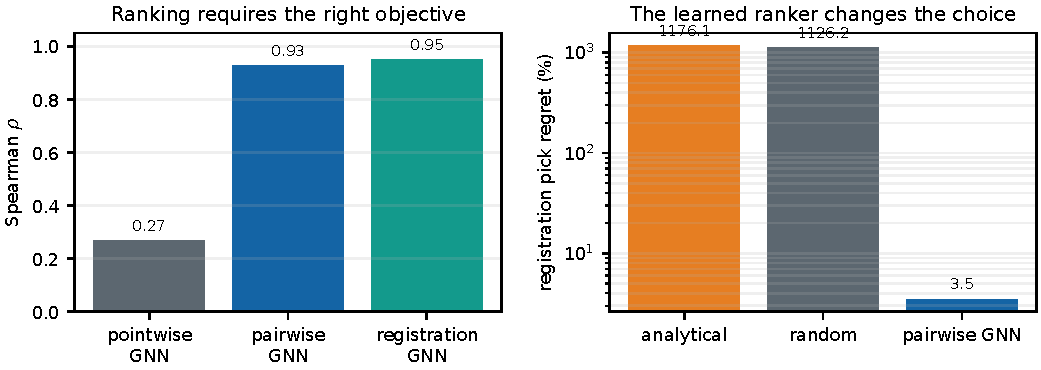
\includegraphics[width=0.94\textwidth]{fig5_ranking_decision.pdf}
\caption{Ranking behavior. A pairwise objective resolves fine within-family order that pointwise regression misses. On lateral registration, the analytical capacitance is position-blind; its selected layout is no better than random, whereas the learned ranker nearly recovers the FEM optimum.}
\label{fig:rank}
\end{figure*}

\subsection{Latency and Speedup}
Figure~\ref{fig:latency} shows why a single number is insufficient. Pre-collated batch throughput is 0.64\,ms/design, but a prepared graph evaluated alone takes 2.37\,ms and the raw-layout path takes 5.90\,ms. The paired FastHenry and FEM reference has a 4.17\,s median, 4.27\,s mean, and 5.36\,s 95th percentile. Describing the reference as ``about 5\,s'' is a coarse summary of this distribution, not an exact constant.

The primary comparison uses the per-design ratio between paired solver time and raw-layout end-to-end inference. Its median is $734.6\times$, with 95\% bootstrap interval $[682.4,795.9]\times$. This is the appropriate speedup for an interactive batch-one path. A historical 1.17\,ms figure came from pre-collated batch throughput and reproduced at 1.33\,ms on the same machine class; combining the rounded 5\,s solver estimate with that throughput yields the familiar approximate $4300\times$, but it is not the primary end-to-end statistic.

Against the analytical implementation, the dense graph is slower at the benchmark's mean size. Sparse $k$-NN inference changes the asymptotic edge count from $O(N^2)$ to $O(Nk)$ and crosses the unaccelerated all-pairs analytical implementation near $N=80$ in the measured scaling study. This crossover concerns runtime; solver-grade accuracy is the reason to use the surrogate below that size.

\begin{figure}[t]
\centering
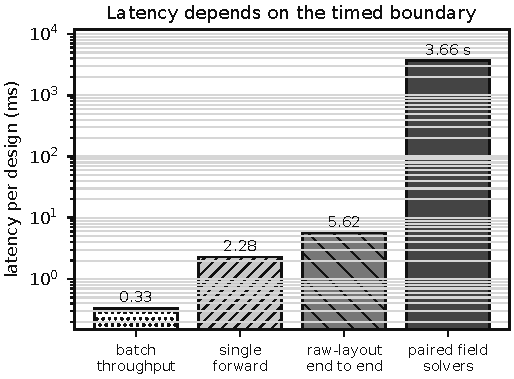
\includegraphics[width=0.98\columnwidth]{fig4_latency_protocols.pdf}
\caption{Measured latency at four timer boundaries. The vertical axis is logarithmic. Pre-collated throughput is useful for a candidate bank, while raw-layout end-to-end time is the conservative batch-one deployment measure.}
\label{fig:latency}
\end{figure}

\begin{table}[t]
\caption{Latency and speedup definitions. All values are medians per design unless noted.}
\label{tab:latency}
\centering
\small
\begin{tabular}{lr}
\toprule
Timed boundary & value\\
\midrule
GNN, pre-collated batch & 0.644\,ms\\
GNN, single prepared graph & 2.372\,ms\\
GNN, raw-layout end to end & 5.900\,ms\\
Paired field solvers & 4.173\,s\\
Paired end-to-end speedup & $734.6\times$\\
95\% speedup interval & $[682.4,795.9]\times$\\
\bottomrule
\end{tabular}
\end{table}

\section{Frequency-Resolved Extension}
The lumped vector does not describe frequency-dependent copper loss. As a separate task, the primary $\Rac/\Rdc(f)$ curve is sampled at 17 logarithmic frequencies from 10\,kHz to 100\,MHz. FastHenry with cross-section subdivision supplies the reference. A 17-output GNN trained on 109 of 136 boards achieves 0.37\% median curve error and $R^2=0.995$ on 27 held-out boards.

Figure~\ref{fig:freq} shows the mean curve rising from approximately one to six across the band. The predicted and reference curves nearly overlap. This experiment demonstrates that the graph representation can support a frequency-indexed output, but it is a smaller corpus with its own split; its metric should not be merged with the four-target field-accuracy result.

\begin{figure}[t]
\centering
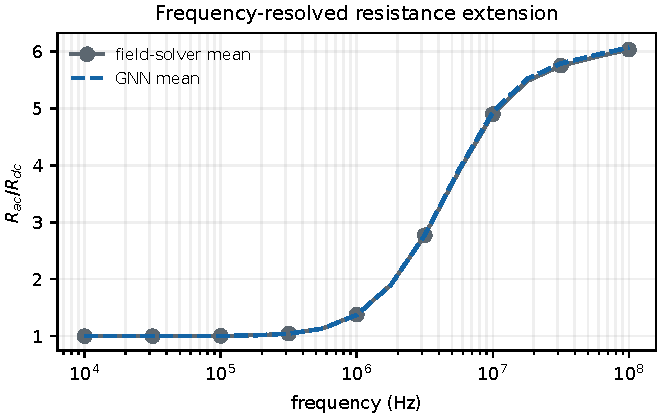
\includegraphics[width=0.98\columnwidth]{fig6_frequency.pdf}
\caption{Mean held-out $\Rac/\Rdc(f)$ curve for the separate frequency-resolved task. The 17-output model attains 0.37\% median curve error over 27 test boards.}
\label{fig:freq}
\end{figure}

\section{Discussion}
\subsection{What the Graph Contributes}
The evidence does not support a blanket statement that a graph is superior for every output. A well-tuned tree ensemble is competitive for typical $\Cps$ error because the capacitance target can be strongly correlated with pooled size and overlap statistics. The graph earns its complexity on the inductive quantities, size transfer, and pairwise decision task. Those are precisely the cases in which relations among traces cannot be compressed safely into fixed global moments.

The same caution applies to equivariance. Exact symmetry is desirable as an implementation guarantee. It removes coordinate-frame dependence from the encoded-graph model and gives a clean transformation contract. Yet the present field corpus does not resolve an accuracy benefit over a strong invariant distance-message network, nor does it establish practical equivalence. More seeds or a benchmark with arbitrary three-dimensional orientations would be required to distinguish effects within roughly nine percent.

\subsection{Deployment in a Design Loop}
The intended workflow is screen, rank, then confirm. The GNN evaluates a broad candidate bank; the pairwise head orders close variants; a field solve confirms a small finalist set. This division avoids using a surrogate as the final sign-off tool. It also makes the latency boundary explicit: batched throughput predicts the cost of a large bank, whereas 5.90\,ms estimates an isolated raw-layout query.

The implementation uses PyTorch without PyG or DGL. The dependency choice simplifies embedding and licensing, although it is not a scientific accuracy claim. Sparse graphs should be selected when trace count is high enough for graph construction and all-pairs messages to matter. For the modest boards in the accuracy corpus, dense connectivity remains a reasonable reference architecture.

\subsection{Limitations}
Four limitations define the next experiment.

First, there is no fabricated-board anchor. FastHenry, the electrostatic FEM, and the independent Neumann calculation establish numerical consistency within a modeled geometry. They do not include connector fixtures, solder, copper roughness, or manufacturing distributions. Impedance or resonant measurements on a controlled PCB coupon are needed before claiming hardware accuracy.

Second, the geometry family is intentionally narrow: rectangular foils in an eight-layer planar winding, without vias, return planes, complex cutouts, or arbitrary curved routing. The strict model is verified only on the graph produced from this family. Extending the raw-layout encoder while preserving a well-defined symmetry action is a separate problem.

Third, the inductances are winding quantities in free space. The ferrite magnetic circuit and its nonlinear, frequency-dependent permeability are not learned. A separate FEM sanity check reproduces an EER40 GP95 datasheet $A_L$ within roughly 4--6\% at representative production gaps, but that validates the core solver, not this GNN.

Fourth, the capacitance FEM uses an effective dielectric description. Layered anisotropic dielectrics, frequency-dependent loss tangent, and full-wave coupling are outside its scope. These omissions matter most when the surrogate is moved from layout ranking to absolute EMI prediction.

\section{Reproducibility and Artifact Organization}
The repository contains the dataset generators, graph and model code, solver interfaces, experiment outputs, and the complete LaTeX source for this manuscript. The numerical source for every new figure is a machine-readable JSON file beside the plotting script. Figure generation is deterministic. A clean build invokes the figure script and runs the LaTeX toolchain from the manuscript directory.

Heavy reference generation is intentionally separated from document building. Recreating the 332-design field corpus requires repeated three-dimensional solves and should run on a managed compute system. Rebuilding the figures and PDF consumes only released result files. External FastHenry and capacitance-solver binaries are not redistributed; their interfaces and build instructions are provided.

\section{Conclusion}
Solver supervision, rather than architectural novelty alone, is the decisive change in this study. Replacing analytical labels reduces held-out median error to 2.56--3.81\% across $\Cps$, $\Lp$, $\Ls$, and $\Mut$, and an independent Neumann formulation bounds the remaining inductive discrepancy. Graph structure matters most for relational targets, size transfer, and fine layout decisions. A pairwise objective turns high absolute accuracy into useful within-family ordering and nearly recovers the optimal lateral-registration choice where the analytical model is blind.

The corrected EGNN supplies strict $E(3)$ behavior on encoded graphs, but its predictive effect remains unresolved against a parameter-matched invariant model. Latency likewise depends on the stated boundary: the conservative raw-layout path is 5.90\,ms/design and gives a paired end-to-end median speedup of $735\times$ over the evaluated field workflow. These are encouraging screening results, bounded by a clear qualification: the surrogate is solver-grade and synthetic-geometry validated. Measured boards, richer layout primitives, layered dielectric references, and joint core-winding models are the next steps.

\appendix
\section{Feature and Symmetry Contract}
Table~\ref{tab:features} records the representation used in the controlled invariant/strict comparison. This contract differs from an earlier exploratory model that passed all seven edge channels, including Cartesian vector components, to an unconstrained MLP. That exploratory model is useful as a counterexample: an EGNN-style coordinate update does not rescue scalar invariance when its message already depends on a coordinate-frame-specific input.

\begin{table*}[t]
\caption{Feature contract for the controlled architecture comparison. ``Invariant'' refers to the encoded-graph $E(3)$ action defined in Section~III-C.}
\label{tab:features}
\centering
\small
\begin{tabular}{p{0.18\textwidth}p{0.31\textwidth}p{0.12\textwidth}p{0.29\textwidth}}
\toprule
Component & channels & transformation & use in both arms\\
\midrule
Node scalars & width, length, thickness, $\log\sigma$, $\epsilon_r$, normalized layer & invariant & encoded to hidden scalar state\\
Node coordinates & normalized $x,y,z$ with one isotropic scale & vector & used to recompute squared distance\\
Edge metadata & overlap, capacitive flag, inductive flag & invariant by test definition & encoded once and held fixed under graph transform\\
Distance & $\|x_i-x_j\|^2$ & invariant & recomputed inside every message layer\\
Coordinate update & bounded scalar weight times $x_i-x_j$ & equivariant & strict arm only\\
Readout & mean, max, signed-log-sum & invariant & shared graph-level pooling\\
\bottomrule
\end{tabular}
\end{table*}

One isotropic coordinate scale is essential. Standardizing $x$, $y$, and $z$ with separate factors maps a rotation to a non-orthogonal transformation in normalized space. The same issue applies to data augmentation: rotating coordinates but leaving a raw relative-vector edge channel unchanged tests a different graph, not the claimed group action.

The symmetry gate uses relative residual
\begin{equation}
\delta_y=\frac{\|f(QX+t)-f(X)\|_2}{\|f(X)\|_2+\varepsilon}
\end{equation}
for graph output and
\begin{equation}
\delta_x=\frac{\|X_L(QX+t)-(QX_L(X)+t)\|_F}{\|QX_L(X)+t\|_F+\varepsilon}
\end{equation}
for coordinates after the last layer. The largest observed values are reported in Table~\ref{tab:egnn}; no rounded prediction percentage is used as the strictness criterion.

\section{Seed-Level Architecture Results}
Table~\ref{tab:seed} exposes the five full-data primary errors rather than presenting only a pooled effect. Strict EGNN is better for two seeds and worse for three. The variation explains the nearly zero mean effect and the broad hierarchical interval. It also prevents a single favorable initialization from being presented as an architectural result.

\begin{table}[t]
\caption{Full-data primary error by initialization seed. Lower is better.}
\label{tab:seed}
\centering
\small
\begin{tabular}{rrr}
\toprule
Seed & invariant, matched & strict EGNN\\
\midrule
42 & 0.031097 & 0.031532\\
43 & 0.030910 & 0.032871\\
44 & 0.027454 & 0.025291\\
45 & 0.028530 & 0.026124\\
46 & 0.026451 & 0.028615\\
\midrule
Mean & 0.028888 & 0.028886\\
\bottomrule
\end{tabular}
\end{table}

At 50 training designs, strict EGNN is practically worse by 11.07\% with 95\% interval $[3.27,19.74]$\%. At 25, 100, and 200 designs the intervals cross zero. These pointwise learning-curve analyses are secondary to the preselected AULC summary, but they show that sample efficiency is not monotonically improved by coordinate updates.

\section{Teacher Fidelity and Solver Accuracy}
The 2000-layout analytical-label corpus remains useful for controlled architecture debugging. On its held-out set, dense message passing reaches $R^2=0.9998$, 0.9996, 0.9995, and 0.9997 for $\Cps$, $\Lp$, $\Ls$, and $\Mut$. A two-layer model is similar to the four-layer model, while removal of relative geometry roughly doubles inductance RMSE. A sparse $k$-NN model retains $R^2\ge0.992$ in the principal four-target comparison.

Those values should be read as fidelity to a deterministic analytical teacher. They answer whether the network can learn the extensive pairwise calculation, not whether the calculation is physically accurate. The field-corpus results in Table~\ref{tab:field} answer the second question. Keeping the two tables separate avoids the misleading inference that $R^2>0.999$ applies against the three-dimensional solvers.

The failed capacitance-BEM route is also retained in the release. Uniform-panel estimates varied by factors of six to forty as panel density changed at the thinnest dielectric gaps, and the resulting corpus produced negative held-out $R^2$. Adaptive refinement improved conditioning but increased solve time substantially. The volume FEM was selected because its conductor regions and dielectric volume yielded stable geometry sensitivity over the required gap range. This is a numerical-method choice, not evidence that volume FEM is universally preferable to BEM.

\section{Additional Timing Interpretation}
The paired solver median is 4.173\,s, while its mean is 4.268\,s and 95th percentile 5.360\,s. The spread comes mainly from the electrostatic mesh and solve; FastHenry is the smaller component for these layouts. Reporting a distribution matters for two reasons. First, a projected bank runtime based on a rounded 5\,s constant is conservative near the median but not a direct measurement of every candidate. Second, ratios of independent medians and medians of paired ratios need not agree.

For this reason the paper's primary $734.6\times$ result is the median of paired per-design solver/end-to-end ratios. Its 95\% interval $[682.4,795.9]\times$ resamples designs. The pre-collated throughput is reported separately and should be used only when graph preparation is outside the timed loop or amortized over a candidate bank. Hardware, thread count, warm-up, batch size, repeat count, and timer boundary remain necessary context when comparing latency with another system.

\bibliographystyle{unsrt}
\bibliography{references}

\end{document}
